{\large(a)}

\textbf{Sobel filter (3 by 3)}

We will use the $3\times3$ Sobel filter to produce image dipicting the edges in the original image:

$$\delta_x = \frac{1}{4}
\begin{bmatrix}
-1 & 0 & 1 \\
-2 & 0 & 2 \\
-1 & 0 & 1
\end{bmatrix}$$

and,

$$\delta_y = \frac{1}{4}
\begin{bmatrix}
-1 & -2 & -1 \\
0 & 0 & 0 \\
1 & 2 & 1
\end{bmatrix}$$

Thus we get the gradients in different directions.

\begin{figure}[H]
    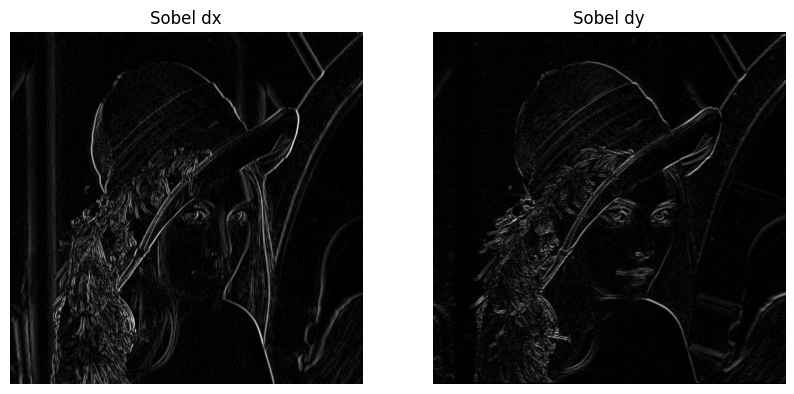
\includegraphics[width=1.06\textwidth]{res/2a_sobel.png}
    \caption{Sobel filter applied to the original image}
    \label{fig:2a_sobel}
\end{figure}

\textbf{Comparision with 5 by 5 Sobel filter}

We will use following $5\times5$ filter to produce image dipicting the edges in the original image:

$$\delta_x = \frac{1}{24}
\begin{bmatrix}
-1 & -2 & 0 & 2 & 1 \\
-2 & -3 & 0 & 3 & 2 \\
-3 & -5 & 0 & 5 & 3 \\
-2 & -3 & 0 & 3 & 2 \\
-1 & -2 & 0 & 2 & 1
\end{bmatrix}$$

and,

$$\delta_y = \frac{1}{24}
\begin{bmatrix}
-1 & -2 & -3 & -2 & -1 \\
-2 & -3 & -5 & -3 & -2 \\
0 & 0 & 0 & 0 & 0 \\
2 & 3 & 5 & 3 & 2 \\
1 & 2 & 3 & 2 & 1
\end{bmatrix}$$

\begin{figure}[H]
    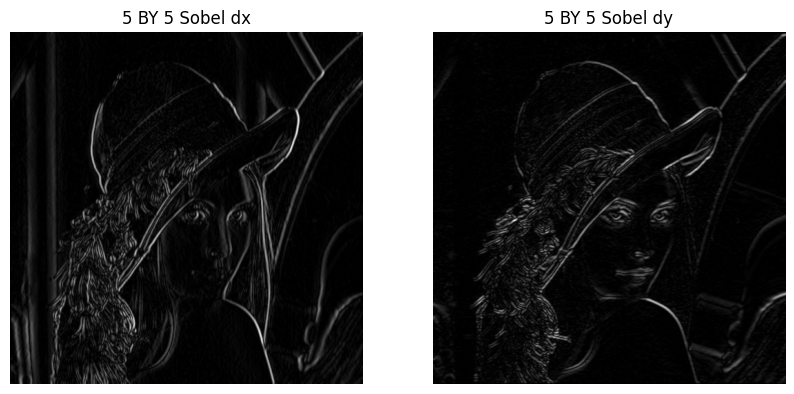
\includegraphics[width=1.06\textwidth]{res/2a_5_by_5.png}
    \caption{Sobel filter (5 by 5) applied to the original image}
    \label{fig:2a_5by5}
\end{figure}


\textbf{Combining the gradients}

We can compute the final gradient using the following formula:

$$
||\delta(I)|| = \sqrt{\delta_x^2 + \delta_y^2}
$$

Here I am basically making a 2d vector out of the two gradients and then taking the magnitude of the vector. This will give us the final gradient image. We have to do this for each corresponding pixels.


\begin{figure}[H]
    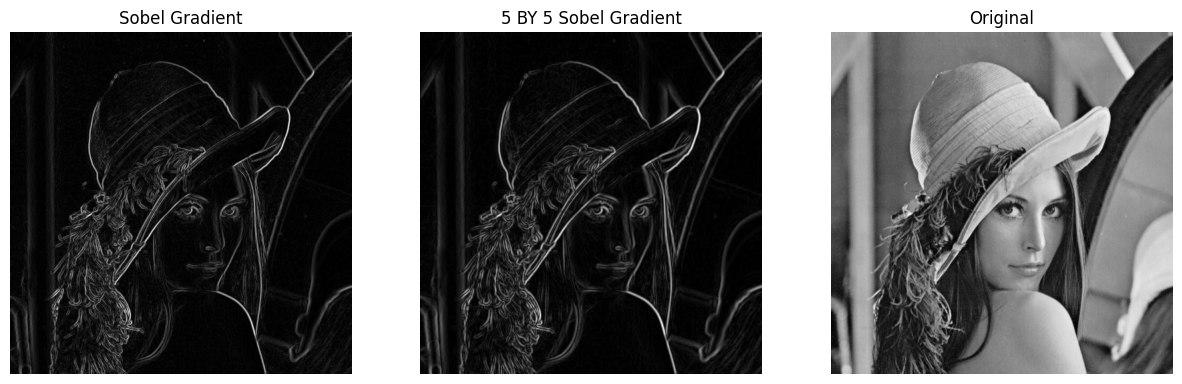
\includegraphics[width=1.06\textwidth]{res/2a_gradient.png}
    \caption{Gradients calculated for different kernel size filters}
    \label{fig:2a_gradient}
\end{figure}

{\large(b)}

\textbf{Results from different kernel sizes}

\begin{itemize}
    \item The details on hair are well preserved in the $3\times3$ filter compared to that of the $5\times5$ filter.
    \item Overall, the result from $5\times5$ filter is around a pixel or two width thicker than that of  $3\times3$ filter.
    \item $5\times5$ takes mroe time to compute than that of $3\times3$.
\end{itemize}


{\large(c)}

\textbf{Thresholding}

Thresholding is a technique used to convert a grayscale image to a binary image. If the pixel value is greater than the threshold value, we set it to 255 (white) else we set it to 0 (black). This will give us a binary image. This is useful in edge detection because we can remove the noise in the image, which may have caused subtle disruptions in the gradient image and only keep the edges.

\begin{figure}[H]
    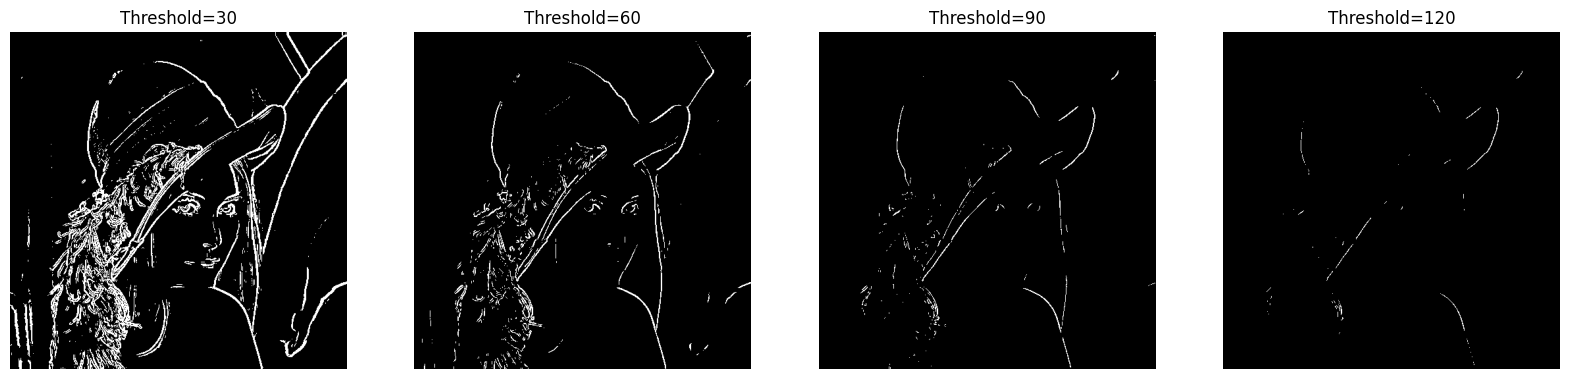
\includegraphics[width=1.06\textwidth]{res/2c_3by3.png}
    \caption{Thresholding applied to the gradient image for Sobel $3\times3$}
    \label{fig:2c_3by3}
\end{figure}

\begin{figure}[H]
    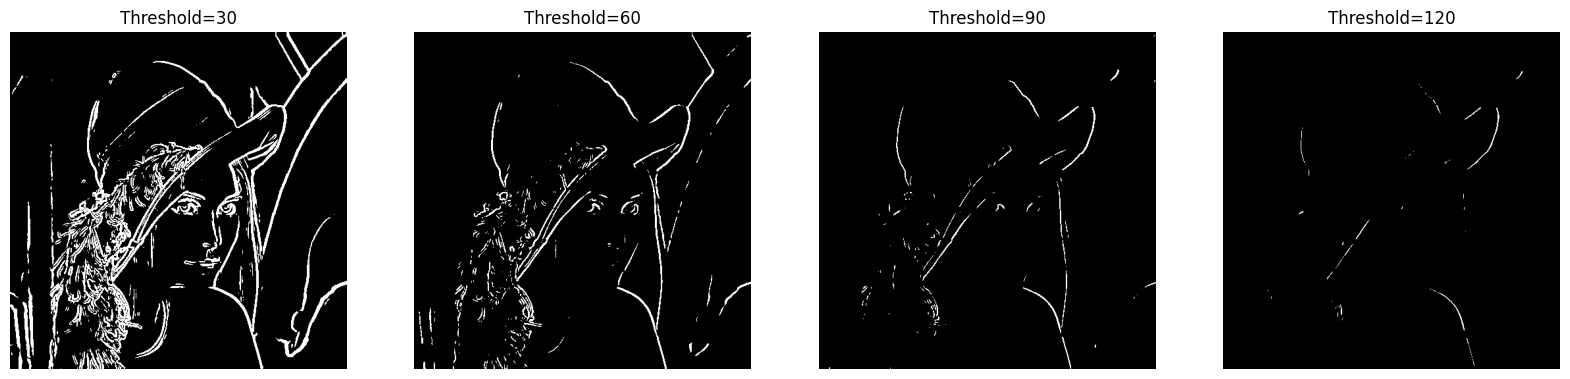
\includegraphics[width=1.06\textwidth]{res/2c_5by5.png}
    \caption{Thresholding applied to the gradient image for Sobel $5\times5$}
    \label{fig:2c_5by5}
\end{figure}

Both the filter gives more or less same results here, appart from the edges are still everso slightly thicker in the $5\times5$ filter.

{\large(d)}

\textbf{Applying noise to the image.}

I added gaussian noise to the image. Here I have experimented with different values of sigma for the noise.

\begin{figure}[H]
    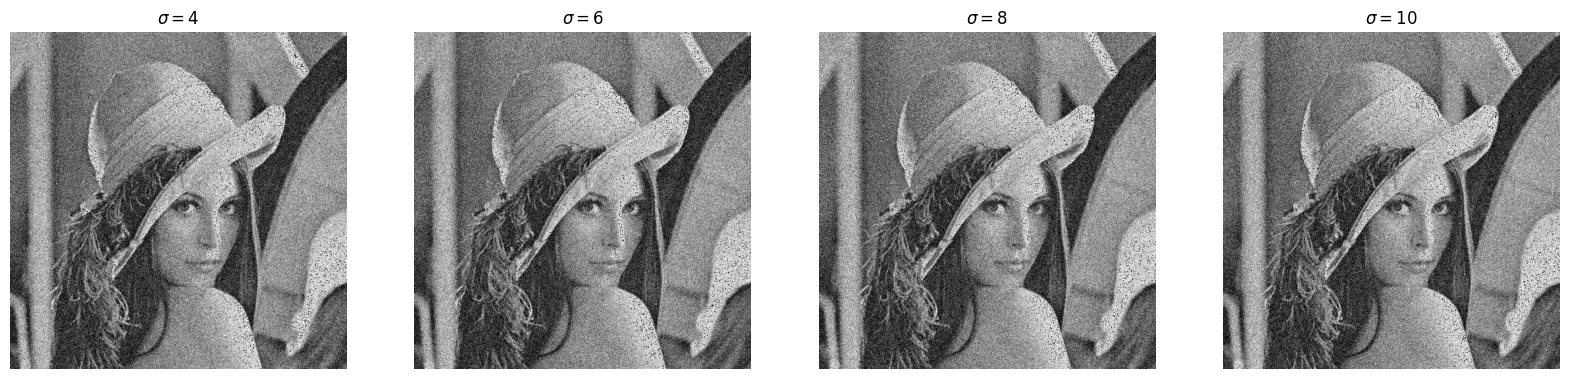
\includegraphics[width=1.06\textwidth]{res/2d_noise.png}
    \caption{Gaussian noise applied different values of sigma}
    \label{fig:2d_noise}
\end{figure}

\textbf{How noise affects edge detection}

Noise in the image heavily impacts the edge detection algorithms we are considering here. The noise in the image causes the gradient image to have a lot of noise. This noise can be seen in the gradient image. This noise can be removed by thresholding, but this will also remove the subtle edges in the image. This is why it is important to have a clean image before applying edge detection algorithms.

\begin{figure}[H]
    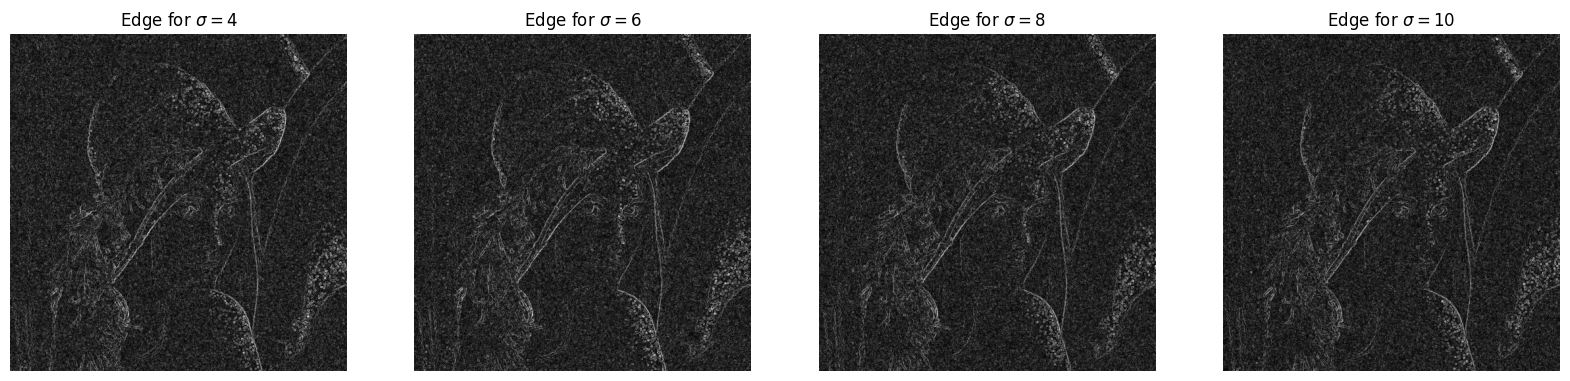
\includegraphics[width=1.06\textwidth]{res/2d_3by3.png}
    \caption{Sobel filter ($3\times3$) applied to the noisy image}
    \label{fig:2d_3by3}
\end{figure}


\begin{figure}[H]
    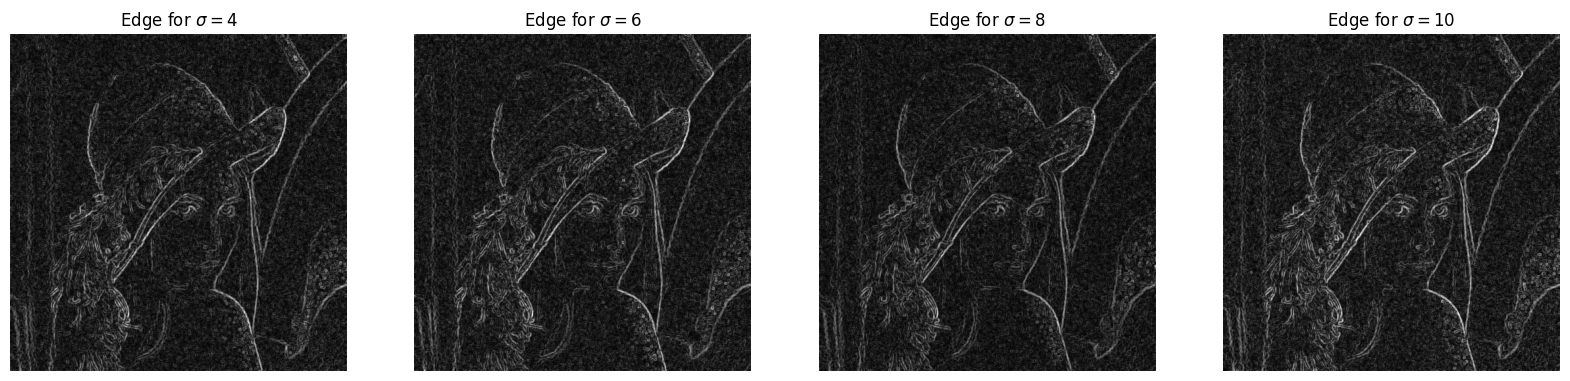
\includegraphics[width=1.06\textwidth]{res/2d_5by5.png}
    \caption{Sobel filter ($5\times5$) applied to the noisy image}
    \label{fig:2d_5by5}
\end{figure}

Here it is easily observed that the noise in the gradient image obtained by the $3\times3$ filter is much more than that of in $5\times5$. Thus impact of noise lowered with larger kernel size. However, both the images are yet noisey, and the edges are not clearly visible. This is why it is important to have a clean image before applying edge detection algorithms.